\begin{figure}[htp]
    \centering
        \begin{subfigure}[b]{\textwidth}
            \centering
          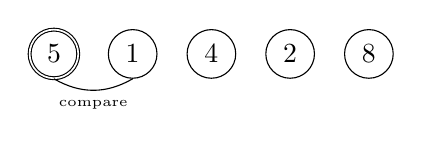
\begin{tikzpicture}
            \path (0,0) node[circle,double,draw] (A) {5};
            \path node[circle,draw,right of=A] (B) {1};
            \path node[circle,draw,right of=B] (C) {4};
            \path node[circle,draw,right of=C] (D) {2};
            \path node[circle,draw,right of=D] (E) {8};
        
            \begin{scope}[every node/.append style={midway}]
              \draw[bend right] (A.south) edge node[below]{\tiny compare} (B.south);
            \end{scope}
          \end{tikzpicture}
        \end{subfigure}
        \begin{subfigure}[b]{\textwidth}
            \centering
              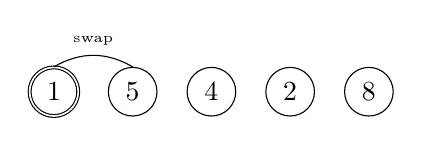
\begin{tikzpicture}
                \path (0,0) node[circle,double,draw] (A) {1};
                \path node[circle,draw,right of=A] (B) {5};
                \path node[circle,draw,right of=B] (C) {4};
                \path node[circle,draw,right of=C] (D) {2};
                \path node[circle,draw,right of=D] (E) {8};
            
                \begin{scope}[every node/.append style={midway}]
                  \draw[bend left] (A.north) edge node[above]{\tiny swap} (B.north);
                \end{scope}
              \end{tikzpicture}
        \end{subfigure}

        \rulesep

        \begin{subfigure}[b]{\textwidth}
            \centering
              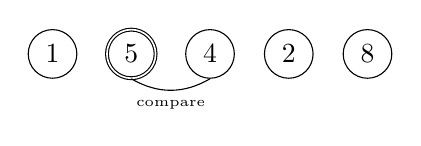
\begin{tikzpicture}
                \path (0,0) node[circle,draw] (A) {1};
                \path node[circle,draw,double,right of=A] (B) {5};
                \path node[circle,draw,right of=B] (C) {4};
                \path node[circle,draw,right of=C] (D) {2};
                \path node[circle,draw,right of=D] (E) {8};
            
                \begin{scope}[every node/.append style={midway}]
                  \draw[bend right] (B.south) edge node[below]{\tiny compare} (C.south);
                \end{scope}
              \end{tikzpicture}
        \end{subfigure}
        \begin{subfigure}[b]{\textwidth}
            \centering
              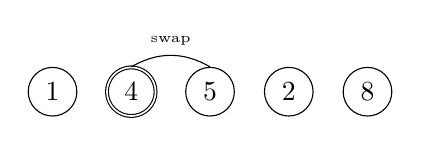
\begin{tikzpicture}
                \path (0,0) node[circle,draw] (A) {1};
                \path node[circle,draw,double,right of=A] (B) {4};
                \path node[circle,draw,right of=B] (C) {5};
                \path node[circle,draw,right of=C] (D) {2};
                \path node[circle,draw,right of=D] (E) {8};
            
                \begin{scope}[every node/.append style={midway}]
                  \draw[bend left] (B.north) edge node[above]{\tiny swap} (C.north);
                \end{scope}
              \end{tikzpicture}
        \end{subfigure}

        \rulesep

        \begin{subfigure}[b]{\textwidth}
            \centering
              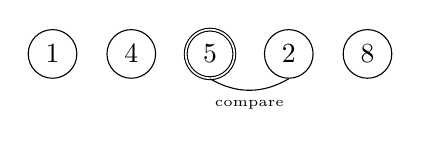
\begin{tikzpicture}
                \path (0,0) node[circle,draw] (A) {1};
                \path node[circle,draw,right of=A] (B) {4};
                \path node[circle,draw,double,right of=B] (C) {5};
                \path node[circle,draw,right of=C] (D) {2};
                \path node[circle,draw,right of=D] (E) {8};
            
                \begin{scope}[every node/.append style={midway}]
                  \draw[bend right] (C.south) edge node[below]{\tiny compare} (D.south);
                \end{scope}
              \end{tikzpicture}
        \end{subfigure}
        \begin{subfigure}[b]{\textwidth}
            \centering
              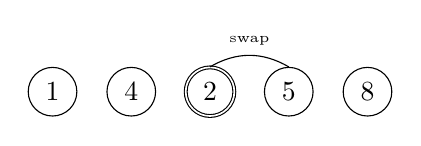
\begin{tikzpicture}
                \path (0,0) node[circle,draw] (A) {1};
                \path node[circle,draw,right of=A] (B) {4};
                \path node[circle,draw,double,right of=B] (C) {2};
                \path node[circle,draw,right of=C] (D) {5};
                \path node[circle,draw,right of=D] (E) {8};
            
                \begin{scope}[every node/.append style={midway}]
                  \draw[bend left] (C.north) edge node[above]{\tiny swap} (D.north);
                \end{scope}
              \end{tikzpicture}
        \end{subfigure}
        
        \rulesep
        
        \begin{subfigure}[b]{\textwidth}
            \centering
              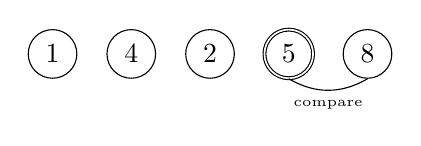
\begin{tikzpicture}
                \path (0,0) node[circle,draw] (A) {1};
                \path node[circle,draw,right of=A] (B) {4};
                \path node[circle,draw,right of=B] (C) {2};
                \path node[circle,draw,double,right of=C] (D) {5};
                \path node[circle,draw,right of=D] (E) {8};
            
                \begin{scope}[every node/.append style={midway}]
                  \draw[bend right] (D.south) edge node[below]{\tiny compare} (E.south);
                \end{scope}
              \end{tikzpicture}
        \end{subfigure}
        \begin{subfigure}[b]{\textwidth}
            \centering
              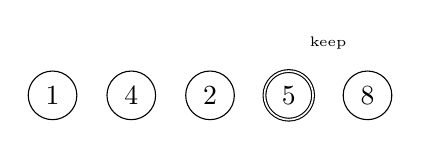
\begin{tikzpicture}
                \path (0,0) node[circle,draw] (A) {1};
                \path node[circle,draw,right of=A] (B) {4};
                \path node[circle,draw,right of=B] (C) {2};
                \path node[circle,draw,double,right of=C] (D) {5};
                \path node[circle,draw,right of=D] (E) {8};
            
                \begin{scope}[every node/.append style={midway}]
                  \draw[bend left] (D.north) edge[draw=none] node[above]{\tiny keep} (E.north);
                \end{scope}
              \end{tikzpicture}
        \end{subfigure}
        
        \rulesep
        
        \begin{subfigure}[b]{\textwidth}
            \centering
              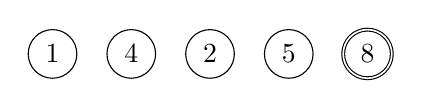
\begin{tikzpicture}
                \path (0,0) node[circle,draw] (A) {1};
                \path node[circle,draw,right of=A] (B) {4};
                \path node[circle,draw,right of=B] (C) {2};
                \path node[circle,draw,right of=C] (D) {5};
                \path node[circle,draw,double,right of=D] (E) {8};
              \end{tikzpicture}
        \end{subfigure}
        \begin{subfigure}[b]{\textwidth}
            \centering
              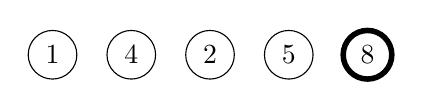
\begin{tikzpicture}
                \path (0,0) node[circle,draw] (A) {1};
                \path node[circle,draw,right of=A] (B) {4};
                \path node[circle,draw,right of=B] (C) {2};
                \path node[circle,draw,right of=C] (D) {5};
                \path node[circle,draw,line width=2pt,right of=D] (E) {8};
              \end{tikzpicture}
        \end{subfigure}
\end{figure}